\chapter{Determinação da constante de propagação}

A constante de propagação do ambiente determinada pela Texas Instruments deve ser definida empiricamente. Portanto, foram tomados dez valores RSSI para distâncias conhecidas, medidas com uma trena, para que pudessem ser verificados os pontos críticos em que pudéssemos nos manter dentro do erro previsto. Além disso, foi medido RSSI consistente de -60 dB para 1 metro de distância.

\begin{table}[ht]
\centering
\caption{Intensidades observadas para cada distância medida com trena}
\vspace{0.5cm}
\begin{tabular}{l|ccccccc}
\hline
Distância (m) & 0,5 & 1,7 & 2,5 & 5 & 7,5 & 10 & 12,5 \vspace{0.4cm}\\

RSSI (dB) & 
\makecell{-56 \\ -57 \\ -62 \\ -56 \\ -55 \\ -58 \\ -61 \\ -62 \\ -63 \\ -63 \\ -63 \\ -63 \\ -63} &
\makecell{-69 \\ -63 \\ -63 \\ -64 \\ -64 \\ -65 \\ -69 \\ -69 \\ -69 \\ -69 \\ -69 \\ -69 \\ -65} &
\makecell{-72 \\ -69 \\ -62 \\ -62 \\ -71 \\ -70 \\ -64 \\ -63 \\ -64 \\ -63 \\ -64 \\ -63 \\ -62} &
\makecell{-86 \\ -79 \\ -77 \\ -79 \\ -81 \\ -82 \\ -82 \\ -81 \\ -81 \\ -80 \\ -80 \\ -81 \\ -81} &
\makecell{-85 \\ -90 \\ -86 \\ -85 \\ -84 \\ -84 \\ -85 \\ -90 \\ -91 \\ -90 \\ -87 \\ -87 \\ -86} &
\makecell{-81 \\ -81 \\ -82 \\ -82 \\ -81 \\ -82 \\ -84 \\ -84 \\ -85 \\ -84 \\ -85 \\ -87 \\ -86} &
\makecell{-84 \\ -89 \\ -96 \\ -96 \\ -90 \\ -93 \\ -90 \\ -95 \\ -95 \\ -94 \\ -98 \\ -96 \\ -97}
\vspace{0.4cm}\\

RSSI médio (dB) & -60,15 & -66,69 & -65,30 & -80,77 & -86,92 & -83,38 & -93,30
\vspace{0.4cm}\\

n & -0,05 & 2,90 & 1,33 & 2,97 & 3,08 & 2,34 & 3,04
\end{tabular}
\end{table}

Assim, tomando o RSSI médio para cada distância, são listados os coeficientes de propagação ideais de cada medida. Tomando a moda de aproximadamente 2,95 e a média de 2,6, foram calculadas as distâncias que seriam medidas para ambos os coeficientes e, então, calculado o erro quadrático em cada ponto.

\begin{figure}[ht]
  \centering
    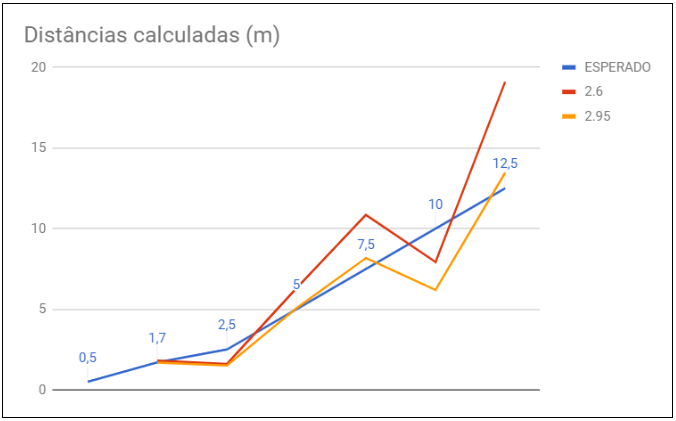
\includegraphics[scale=0.916]{graph-dist}
  \caption{Gráfico das distâncias calculadas para cada n (Fonte: autores)}
\end{figure}

\begin{figure}[ht]
  \centering
    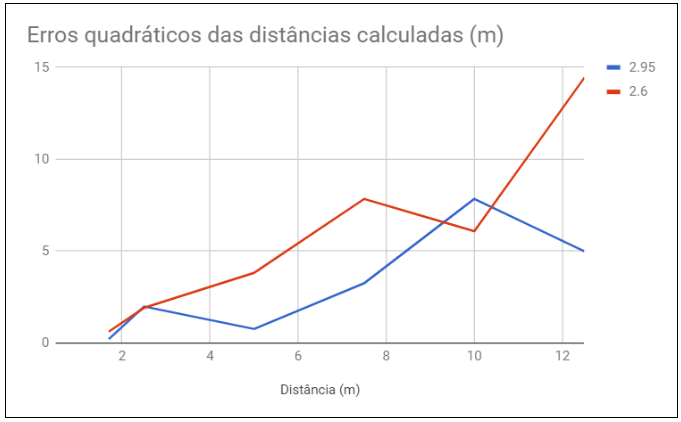
\includegraphics[scale=0.92]{graph-erro}
  \caption{Gráfico do erro quadrático para cada n (Fonte: autores)}
\end{figure}

\begin{table}[ht]
\centering
\caption{Erro quadrático médio e máximo para cada n}
\vspace{0.5cm}
\begin{tabular}{l|cc}
\hline
n & 2,95 & 2,6 \vspace{0.4cm}\\
Erro quadrático médio (m) & 2,82 & 4,06 \vspace{0.4cm}\\
Erro quadrático máximo (m) & 7,84 & 7,84
\end{tabular}
\end{table}

Por fim, concordou-se em utilizar o valor de n=2,95 por apresentar menor erro.

O processo realizado para a determinação do coeficiente de propagação poderia ser automatizado com algoritmos que inclusive considerassem mais valores caso fosse interessante expandir a aplicação dessa forma, por exemplo, anexando sonares aos pontos de acesso.